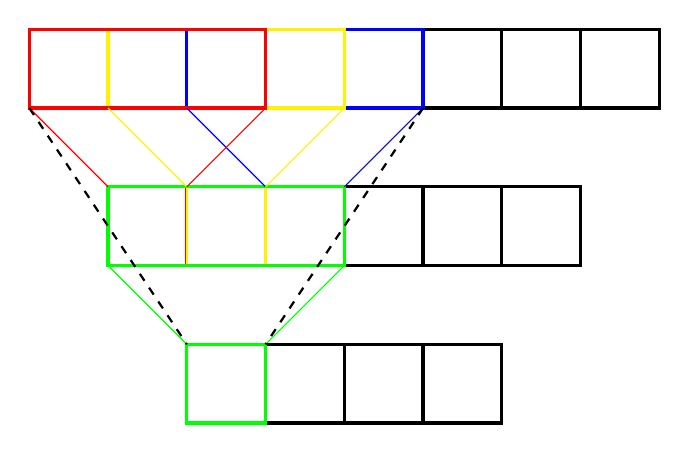
\begin{tikzpicture}[
neuron/.style={circle, draw=black, very thick, minimum size=1cm, transform shape},
dot/.style={circle, draw=black, fill=black, minimum size=0.1cm, inner sep=0pt, transform shape},
note/.style={circle, draw=black, minimum size=0pt, inner sep=0pt, transform shape},
]
%Layer 1
\draw[black, very thick] (0,  0) rectangle (1, -1);
\draw[black, very thick] (1,  0) rectangle (2, -1);
\draw[black, very thick] (2,  0) rectangle (3, -1);
\draw[black, very thick] (3,  0) rectangle (4, -1);
\draw[black, very thick] (4,  0) rectangle (5, -1);
\draw[black, very thick] (5,  0) rectangle (6, -1);
\draw[black, very thick] (6,  0) rectangle (7, -1);
\draw[black, very thick] (7,  0) rectangle (8, -1);

%Filter boxes layer 1
\draw[blue, very thick] (2,  0) rectangle (5, -1);
\draw[yellow, very thick] (1, 0) rectangle (4, -1);
\draw[red, very thick] (0, 0) rectangle (3, -1);

%Layer 2
\draw[red, very thick] (1, -2) rectangle (2, -3);
\draw[blue, very thick] (3, -2) rectangle (4, -3);
\draw[yellow, thick] (2, -2) rectangle (3, -3);
\draw[black, very thick] (4, -2) rectangle (5, -3);
\draw[black, very thick] (5, -2) rectangle (6, -3);
\draw[black, very thick] (6, -2) rectangle (7, -3);

%Filter box layer 2
\draw[green, very thick] (1, -2) rectangle (4, -3);

%Layer 3
\draw[black, very thick] (3, -4) rectangle (4, -5);
\draw[black, very thick] (4, -4) rectangle (5, -5);
\draw[black, very thick] (5, -4) rectangle (6, -5);
\draw[green, very thick] (2, -4) rectangle (3, -5);

%Connections layer 1 -- layer 2
\draw[blue] (2, -1) -- (3, -2);
\draw[blue] (5, -1) -- (4, -2);
\draw[yellow] (1, -1) -- (2, -2);
\draw[yellow] (4, -1) -- (3, -2);
\draw[red] (0, -1) -- (1, -2);
\draw[red] (3, -1) -- (2, -2);

%Connections layer 2 -- layer 3
\draw[green] (1, -3) -- (2, -4);
\draw[green] (4, -3) -- (3, -4);

%Receptive field connections
\draw[black, dashed, thick] (0, -1) -- (2, -4);
\draw[black, dashed, thick] (5, -1) -- (3, -4);
\end{tikzpicture}